\documentclass[a4paper, 12pt]{article}%тип документа

%отступы
\usepackage[left=2cm,right=2cm,top=2cm,bottom=3cm,bindingoffset=0cm]{geometry}

%Русский язык
\usepackage[T2A]{fontenc} %кодировка
\usepackage[utf8]{inputenc} %кодировка исходного кода
\usepackage[english,russian]{babel} %локализация и переносы

%Вставка картинок
\usepackage{graphicx}
\graphicspath{{pictures/}}
\DeclareGraphicsExtensions{.pdf,.png,.jpg}

%Графики
\usepackage{multirow}
\usepackage{pgfplots}
\pgfplotsset{compat=1.9}

%Римские цифры
\newcommand{\RNumb}[1]{\uppercase\expandafter{\romannumeral #1\relax}}

%Математика
\usepackage{amsmath, amsfonts, amssymb, amsthm, mathtools}

%Заголовок
\author{Богданов Александр \\
	Б05-003}
\title{\textbf{Работа 5.8.1 \\ 
		Определение постоянных Стефана-Больцмана и Планка из анализа теплового излучения накаленного тела}}

\begin{document}

\maketitle

\textbf{Цель работы:} 

\begin{enumerate}

    \item При помощи модели абсолютно чёрного тела проведение измерения температуры оптическим пирометром с исчезающей нитью и термопарой.
    
    \item Исследование излучений накалённых тел с различной испускательной способностью.
    
    \item Определение постоянных Планка и Стефана-Больцмана.
    
\end{enumerate}

\textbf{В работе используются:} оптический пирометр,  модель абсолютно чёрного тела,  образцы колец,  вольфрамовая лампа,  неоновая лампа,  блок питания,  цифровые вольтметры.\\

\textbf{Теоретические положения:}\\\par

Для измерения температуры разогретых тел, удаленных от наблюдателя, применяют методы оптической пирометрии, основанные на использовании зависимости испускательной способности исследуемого тела от температуры. Различают три температуры, функционально связанные с истинной термодинамической температурой и излучательной способностью тела: радиационную $T_{\text{рад}}$,  цветовую $T_{\text{цв}}$ и яркостную $T_{\text{ярк}}$. \par

В работе измеряется яркостная температура.  Яркостная температура -- это температура абсолютно чёрного тела,  при которой его спектральная испускательная способность равна спектральной испускательной способности исследуемого тела при той же длине волны.  Измерение яркостной температуры раскалённого тела производится при помощи оптического пирометра с исчезающей нитью, основанного на визуальном сравнении яркости раскалённой нити с яркостью изображения исследуемого тела. \par

Яркостная температура тела всегда ниже его термодинамической температуры.  Это связано с тем,  что любое не чёрное тело излучает меньше, чем АЧТ при той же температуре.  Зависимость между яркостной и термодинамической температурами вольфрама приведена на рис. 1

\begin{figure}[ht]
    \centering
    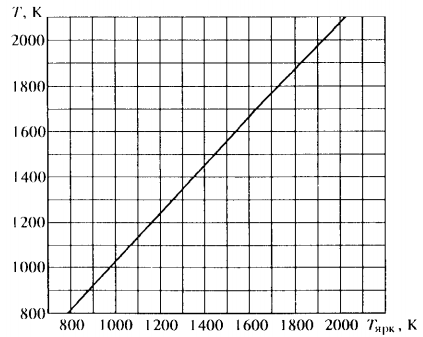
\includegraphics[width=10cm]{График1.PNG}
    \caption{График зависимости $T = f(T_{\text{ярк}})$ для вольфрама}
\end{figure}

\newpage

По результатам измерений мощности излучения вольфрамовой нити можно судить о справедливости закона Стефана-Больцмана.  Если бы нить излучала как АЧТ, то баланс потребляемой и излучаемой энергии определялся бы соотношением:

\[ W = \sigma S (T^4 - T_0^4),\]

где $W$ -- потребляемая нитью электрическая мощность,  $S$ -- площадь излучающей поверхности нити,  $T$ -- температура нити,  $T_0$ -- температура окружающей среды.  Однако вольфрамовая нить излучает как серое тел,  и излучение её ослаблено по сравнению с АЧТ в $\varepsilon_T$ раз для любой волны при данной температуре тела Т.  Тогда предположив, что нить излучает как серое тело и с учётом того, что $T_0 \ll T$, выражение можно переписать в виде:

\[W = \varepsilon_T S \sigma T^4\]
    
В справедливости закона Стефана-Больцмана можно убедиться, построив график зависимости $W(T)$ в логарифмическом масштабе и по углу наклона определить показатель степени $n$ исследуемой температурной зависимости. В пределах погрешности показатель степени должен быть близок к четырём.  Также из формулы  можно определить постоянную Стефана-Больцмана.\\

\textbf{Экспериментальная установка:}

\begin{figure}[ht]
    \centering
    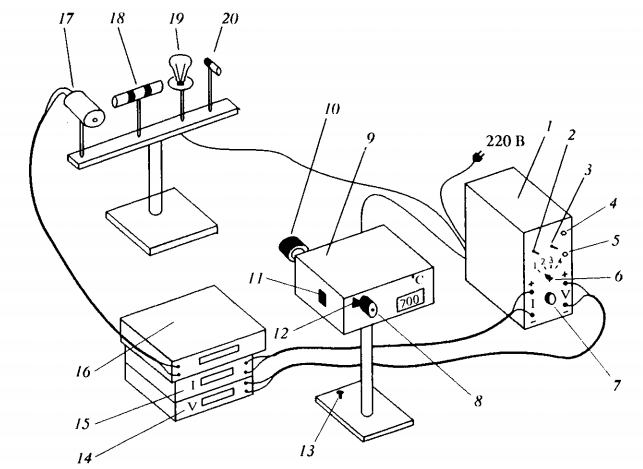
\includegraphics[width=11cm]{Схема.PNG}
    \caption{Схема экспериментальной установки: 1 - блок питания; 2 - тумблер включения питания образцов; 3 - тумблер нагрева нити пирометра; 4 - кнопка "Нагрев нити"; 5 - кнопка "охлаждение нити"; 6 - тумблер переключения образцов; 7 - регулятор мощности нагрева образцов; 8 - окуляр пирометра; 9 - корпус пирометра; 10 - объектив пирометра; 11 - переключение диапазонов; 12 - ручка смещения красного светофильтра; 13 - регулировочный винт; 14 - вольтметр (напряжение на лампе накаливания); 15 - амперметр (ток через образцы); 16 - вольтметр в цепи термопары; 17 - модель АЧТ; 18 трубка с кольцами из материалов с различной излучательной способностью; 19 - лампа накаливания; 20 - неоновая лампочка}
\end{figure}

\newpage

Исследуемые образцы:

\begin{enumerate}

    \item Модель абсолютно чёрного тела -- керамическая трубка,  закрытая с одного конца и окружённая для теплоизоляции внешним кожухом. Температура в трубке измеряется с помощью термопары хромель-алюмель.
    
    \item Керамическая трубка с набором колец из различных материалов, нагреваемая изнутри нихромовой спиралью.  Материалы колец имеют различную излучательную способность.
    
    \item Вольфрамовая нить электрической лампочки.
    
\end{enumerate}

\textbf{Ход работы:}

\begin{enumerate}

\item \textbf{Изучение оптического пирометра}

С помощью пирометра измерим температуры АЧТ и проведем сравнение ее значения со значением температуры,  измеренной при помощи термопарного термометра.

\begin{enumerate}

\item Настроим установку,  прогреем нить,  прогреем модель АЧТ,  введем красный светофильтр пирометра.  Изменяя ток через нить пирометра,  добьемся исчезновения нити на фоне изображения раскаленной поверхности дна АЧТ.

\item По шкале пирометра определим значения яркостной температуры АЧТ.  Также при помощи хромель-алюмелевой термопары и цифрового вольтметра определим температуру модели АЧТ.  Постоянная термопары равна $41\text{мкВ}/^\circ$C,  а комнатная температура равна $20^\circ$C.

\begin{figure}[ht]
    \centering
    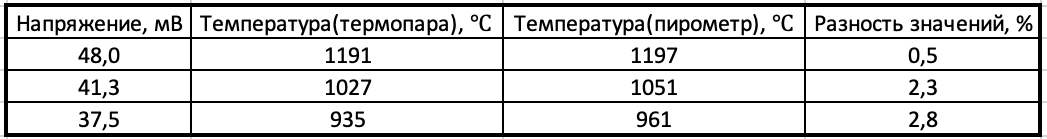
\includegraphics[width=13cm]{Таблица1.PNG}
\end{figure}

Как видно из таблицы относительная погрешность не превышает $2,8 \%$.  Следовательно пирометр работает исправно.

\end{enumerate}

\item \textbf{Измерение яркостной температуры накаленных тел}

Убедимся,  что различные тела,  накаленные до одинаковой термодинамической температуры,  имеют различную яркостную температуру.

Нагреем трубку до темно-красного каления и измерим температуру поверхности трубки и колец.

\begin{figure}[ht]
    \centering
    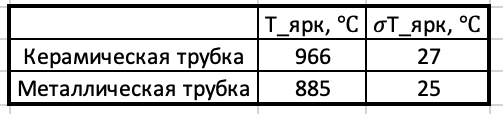
\includegraphics[width=8cm]{Таблица2.PNG}
\end{figure}

Несовпадение яркостной температуры у различных тел,  имеющих одинаковую термодинамическую температуру связано с тем, что эти две величины связаны.

\item \textbf{Проверка закона Стефана - Больцмана}

\begin{enumerate}

\item Постепенно увеличивая накал нити лампы,  измерим пирометром яркостную температуру.  При каждом измерении температуры,  будем записывать величины тока и падения напряжения на нити лампы.

\item Для каждого значения яркостной температуры найдем термодинамическую температуру вольфрамовой нити лампы,  а также посчитаем мощность,  потребляемую нитью лампы.

\begin{figure}[ht]
    \centering
    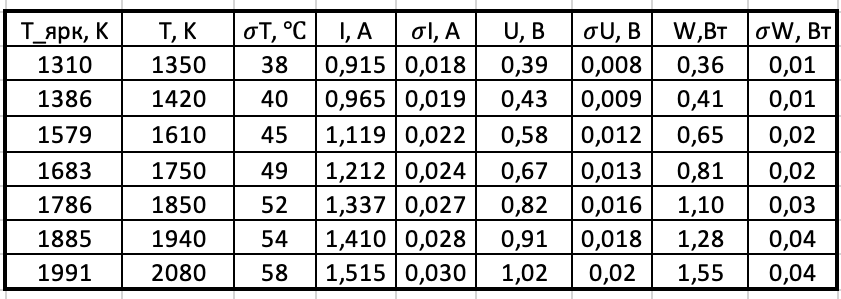
\includegraphics[width=10cm]{Таблица3.PNG}
\end{figure}

\item Построим график $W = f(T)$:

\begin{figure}[ht]
    \centering
    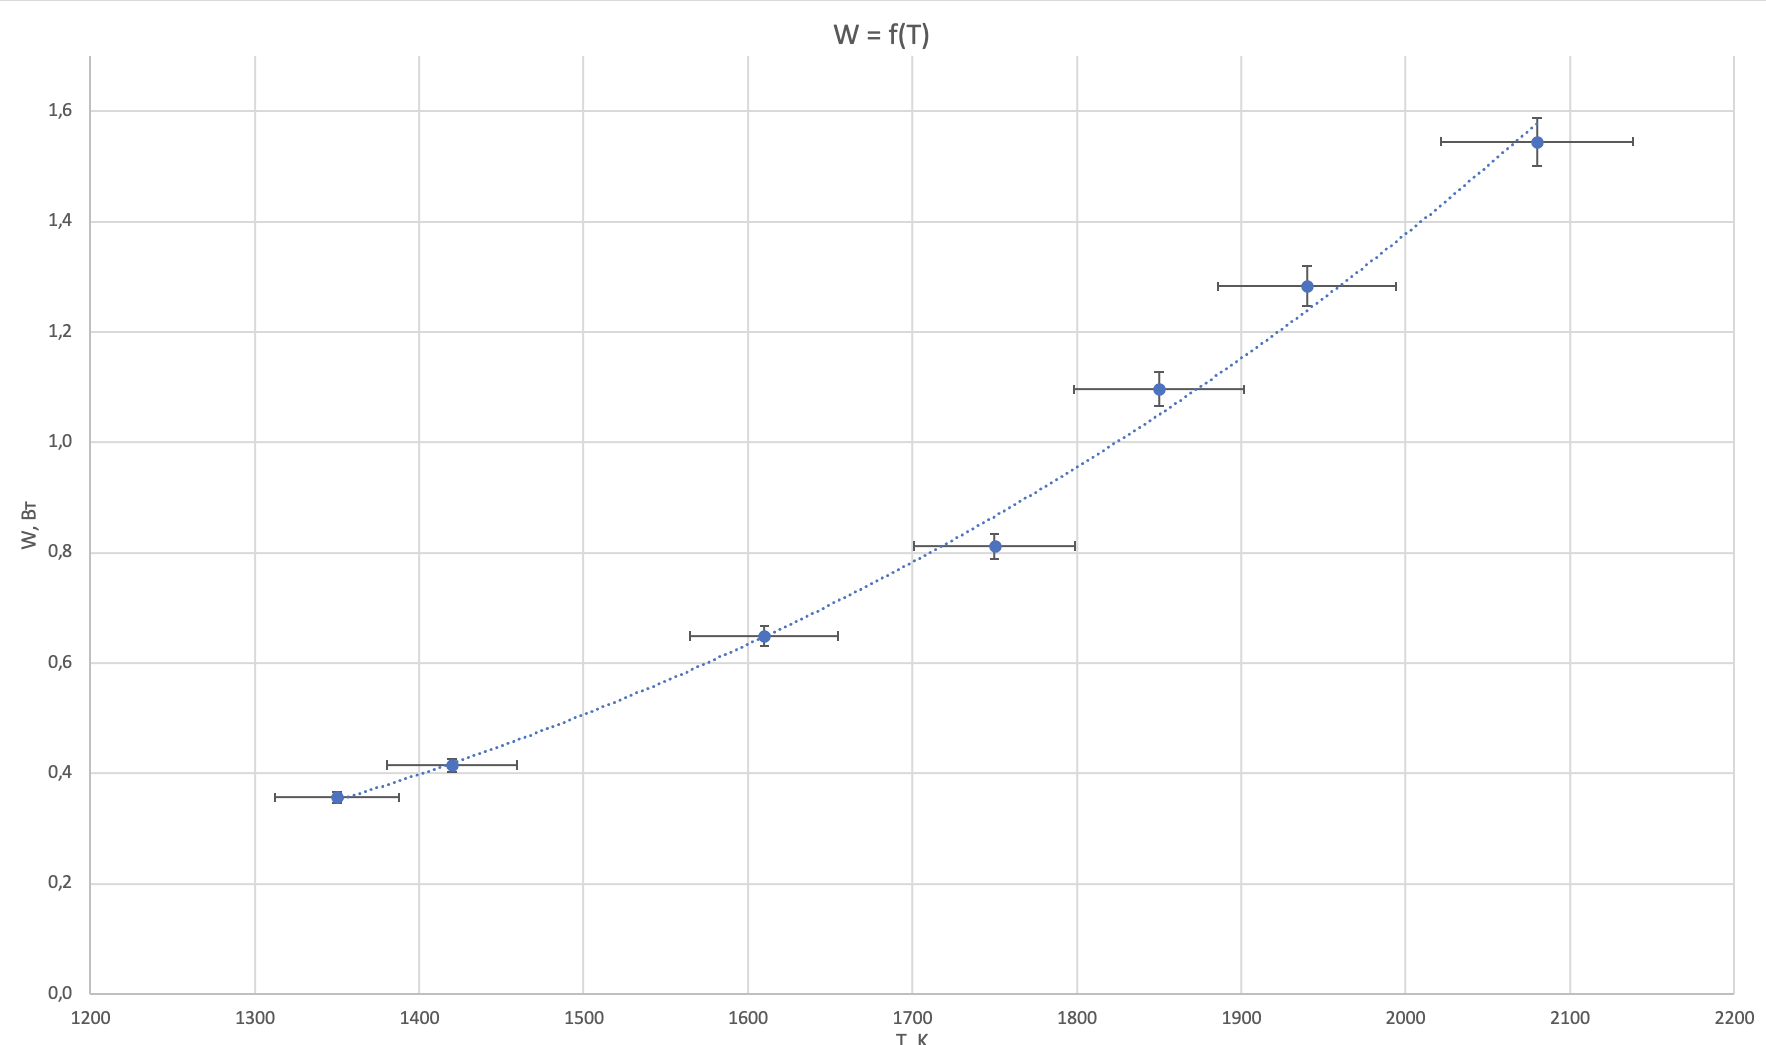
\includegraphics[width=12cm]{График2.PNG}
\end{figure}

\newpage

\item Представим зависимость $W= f(T)$ в логарифмическом масштабе как $\ln(W) = \ln(\varepsilon_T \sigma S) + n \ln(T)$.  По углу наклона графика определим показатель степени температуры в законе Стефана-Больцмана:

\begin{figure}[ht]
    \centering
    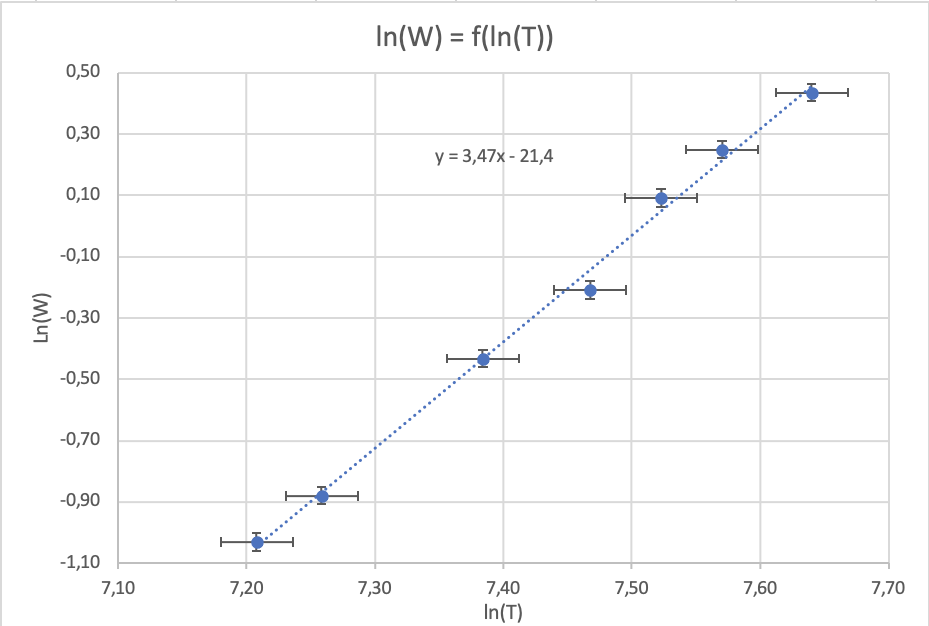
\includegraphics[width=12cm]{График3.PNG}
\end{figure}

По углу наклона определяем показать степени: $3,47 \pm 0, 44$ при теоретическом значении 4.

\item Определим постоянную Стефана-Больцмана, используя значение термодинамической температуры 1850K и соответствующую мощность ($\varepsilon_T(1850) \approx 0.233$, $S = 0.36$ см$^2$):

\begin{center}

\[\sigma = \frac{W}{\varepsilon_T S T^4} = (1, 32 \pm 0,12) \cdot 10^{-12} \text{ Вт}/(\text{см}^2 \cdot K^4)\]

\end{center}

Также можно определить постоянную Стефана-Больцмана, используя построенный график зависимости $\ln(W) = \ln(\varepsilon_T \sigma S) + n \ln(T)$

\begin{center}

\[\ln(\varepsilon_t \sigma S) = -21,4 \pm 0,9\] 
   
\[\sigma = \frac{e^{-21.4}}{\varepsilon_T S} = (1, 71 \pm 0,15) \cdot 10^{-12} \text{ Вт}/(\text{см}^2 \cdot K^4)\]
    
\end{center}

\item Оценим значение постоянной Планка:

\begin{center}

\[h = \sqrt[3]{\frac{2 \pi^5 k_B^4}{15 c^2 \sigma}} \approx (0,91 \pm 0,15) \cdot 10^{-26} \text{ эрг} \cdot \text{с}\]
    
\end{center}

\end{enumerate}

\item \textbf{Измерение яркостной температуры неоновой лампочки}

Термодинамическая температура неоновой лампочки примерно равна комнатной, и не соответствует её яркостной температуре ($\approx$ 868$^{\circ}$C).  Неоновая лампочка не является моделью абсолютно чёрного или серого тела,  и её излучение носит совершенно другую природу. 

\end{enumerate}

\textbf{Вывод:}\\\par

В ходе работы было изучено тепловое излучение модели абсолютно чёрного тела и моделей серых тел - колец из различных материалов и вольфрамовой нити. Было проведено ознакомление с принципом работы оптического пирометра. \par

При проведении работы мы наблюдали, что для различных материалов с одинаковой термодинамической температурой их яркостная температура может не совпадать. \par

В работе было предложено проверить справедливость закона Стефана-Больцмана ($W \propto T^4$).  Данную зависимость удалось получить  -- значение степени при Т составляет $(3.47 \pm 0,44)$,  что совпадает в пределах погрешности с 4.\par

Также по результатам измерений была оценена постоянная Стефана-Больцмана двумя способами: с помощью формулы и используя график зависимости $W(T)$ в логарифмическом масштабе.  Второй способ оказался более точным:

\begin{center}

\[\sigma_1 = (1, 32 \pm 0,12) \cdot 10^{-12} \text{ Вт}/(\text{см}^2 \cdot K^4)\]
\[\sigma_2 = (1, 71 \pm 0,15) \cdot 10^{-12} \text{ Вт}/(\text{см}^2 \cdot K^4)\]
\[\sigma_\text{теор} = 5.67 \cdot 10^{-12} \text{ Вт}/(\text{см}^2 \cdot K^4)\]
     
\end{center}\par

С помощью $\sigma$ мы смогли получить постоянную Планка:

\[h =(0,91 \pm 0,15) \cdot 10^{-26} \text{ эрг} \cdot \text{с}\]
\[h_\text{теор} = 0,66 \cdot 10^{-26} \text{ эрг} \cdot \text{с}\]

В ходе работы с помощью пирометра была определена "яркостная температура" неоновой лампочки,  не являющейся моделью АЧТ.  Эта яркостная температура не совпадает с термодинамической.

\end{document}